\documentclass[10pt]{article}

\usepackage{amsmath}
\usepackage{amssymb}
\usepackage{amsthm}
\usepackage[english]{babel}
\usepackage{graphicx} %figures 
\usepackage{csquotes} %recommended package with bib LaTeX
% \usepackage[style=alphabetic, sorting=ynt]{biblatex} 
\usepackage{faktor} %nicer quotient 
\usepackage{tabularx} %fancy tables
\usepackage{stmaryrd} % lightning symbol 
\usepackage{subcaption} % multiple figures in the same picture
\usepackage{hyperref} % nicer hyperlinks in the text
\usepackage{bbm} %mathbbm 1 command
\usepackage{enumerate} %stylizing enumerate

\newcommand{\bbZ}{\mathbb{Z}}
\newcommand{\bbR}{\mathbb{R}}
\newcommand{\bbF}{\mathbb{F}}
\newcommand{\bbS}{\mathbb{S}}

\newcommand{\ccH}{\mathcal{H}}
\newcommand{\ccO}{\mathcal{O}}

\newcommand{\hmaps}[3][\bbZ_2]{\left[#2, #3\right]_{#1}}
\newcommand{\ztwo}{\bbZ_2}
\newcommand{\hsimp}[3][2]{\mbox{hSimp}_{#1}\left(#2, #3\right)}
\newcommand{\simp}[3][2]{\mbox{Simp}_{#1}\left(#2, #3\right)}
\newcommand{\rar}{\rightarrow}

\newcommand{\scalar}[2]{\left( #1 \vert #2\right)}
\newcommand{\matrice}[1]{\begin{pmatrix}#1\end{pmatrix}}
\newcommand{\norm}[1]{ \lVert #1 \rVert}
\newcommand{\gen}[1]{ \left\langle #1 \right\rangle}

\newtheorem{theorem}{Theorem}
\newtheorem{lemma}{Lemma}
\newtheorem{question}{Question}
\newtheorem{definition}{Definition}

%change \varepsilon to be he default choice
\let\uglyepsilon\epsilon
\let\epsilon\varepsilon



\title{Notes on equipartitions}
\addbibresource{ref.bib}
\author{}

\begin{document}
\maketitle
\graphicspath{{./figs/}}

\section{Notation}
\begin{itemize}
\item Given two vectors $x, y$ of dimension $d$,  their scalar product is $\scalar{x}{y}:=\sum_{i=1}^d x_iy_i$.
\item $G=\bbZ_2\times\bbZ_2$ with elements $\nu_1, \nu_2$ and $\nu_1\nu_2 = \nu_2\nu_1$.
  \item Given a set of elements $S$ in an object $A$ (group elements in a group, vectors in a vector space, etc.), by $\langle S\rangle\subseteq A$ we denote the generated object (group, vector subspace, etc.).
  \item Given a normed vector space $V$, $S(V)$ will denote its sphere
  \item $\bbS_k$ is the group of permutations on $k$ elements and $\bbS_k^{\pm} = \left( \ztwo \right)^k \rtimes \bbS_k$ the signed permutation group.
  \item $G$ acts on $T^2 = S^1\times S^1$ coordinate-wise, i.e.
    \begin{align*}
      \nu_1^T((\theta, \phi)) = (\theta + \pi, \phi) \\
      \nu_2^T((\theta, \phi)) = (\theta, \phi + \pi)
    \end{align*}
  \item $G$ acts on $\bbR^2$ linearly:
    \begin{align*}
      \nu_1(x,y) = (x, -y)\\
      \nu_2(x,y) = (-x, -y)
    \end{align*}
  \item The previous action can be restricted to an action on $S^1=S(\bbR^2)$:
    \begin{align*}
      \nu_1^S(\theta) = 2\pi - \theta \\
      \nu_2^S(\theta) = \theta + \pi
    \end{align*}
  \item An arrangement of planes in $\bbR^3$ is a point $\mathcal{H} \in \left(S^3\right)^3$
    \[
      \mathcal{H}=(\matrice{h_1\\a_1},\matrice{h_2\\a_2}, \matrice{h_3\\a_3})
    \]
  \item Given $\omega \in \left(\ztwo\right)^3$ and an arrangement $\mathcal{H}$, denote by $\mathcal{O}(\mathcal{H}, \omega)$ the open orthant of $\bbR^3$ corresponding to the sign pattern $\omega$; i.e.:
    \[
      \mathcal{O}(\mathcal{H}, \omega) = \left\{ x\in \bbR^3 \  \vert \ (-1)^{\omega_i}\scalar{h_i}{x} > (-1)^{\omega_i}a_i \right\}
    \]
  \item A measure on $\bbR^d$ is nice if it is a Borel probability measure that has a continuous density function with compact connected positive support.
  \item Given a nice measure $\mu$ and $\alpha \in \left(\ztwo\right)^3 \setminus \left\{0\right\}$, the alternating sum defined by $\alpha$ is the function $f_\alpha:(S^3)^3\rightarrow \bbR$:
    \[
      f_\alpha(\mathcal{H}) = \sum_{\beta\in \left(\ztwo\right)^3} (-1)^{\scalar{\alpha}{\beta}}\mu(\mathcal{O}(\mathcal{H}, \beta))
    \]
  \item Fix $\alpha\in \left(\ztwo\right)^k\setminus \left\{0\right\}$, it is possible to define an action of $\left(\ztwo\right)^k$ on $\bbR$ by:
    \[
      \omega(v) = (-1)^{\scalar{\omega}{\alpha}}v
    \]
    Denote by $V_\alpha$ the resulting $\left(\ztwo\right)^k$ representation.
  \item The signed sum maps are $\left(\ztwo\right)^3$-equivariant maps. More precisely, given $\omega, \alpha \in \left(\ztwo\right)^3$ with $\alpha \neq 0$:
    \[
      f_\alpha(\omega \mathcal{H}) = (-1)^{\scalar{\alpha}{\omega}}f_\alpha(\mathcal{H})
    \]
\end{itemize}

The goal of this notes is to prove the following result:
\begin{theorem}
  Let $\mu$ be a nice measure on $\bbR^3$ and $\vec{x} \in S^2$ a direction. Then there exists a triple of affine planes $ \mathcal{H}=(h_1, h_2, h_3) \in (S^3)^3$ and a vector $b\in \bbR^3$ such that:
  \begin{itemize}
  \item For all orthants $\mathcal{O}(\mathcal{H}, \omega)$, $\mu(\mathcal{O}(\mathcal{H}, \omega)) = \frac{1}{8}$
  \item $h_1 \cap h_2 = \bbR \vec{x} + b$
  \end{itemize}
\end{theorem}

\section{Reduction to equivariant topology}\label{sec:torus_conf_space}
The goal of this section is to show that a suitable Configuration Space/Test Map scheme for the problem is $T^2$ with a $G$-map $f:T^2 \rightarrow \bbR^2$. More precisely, we will first construct a test space $E$ and then show that $E$ is $G$-homeomorphic to the torus with the standard $G$-action.

\vskip 1em
Without loss of generality we can assume the direction we want the two planes to intersect is the $\vec{z}$ axis.
Project the mass on the $xy$ plane to obtain a nice measure $\mu^\#$ on $\bbR^2$. The following bisecting lemma applies:

\begin{lemma}[Bisecting]
  Let $\mu^\#$ be a nice measure on $\bbR^2$ and $v\in S^1$ a direction. Then there exists two oriented affine lines $l_0 =\bbR\vec{l_0} + a_0$ and $l_1 = \bbR\vec{l_1} + a_1$ in $\bbR^2$ such that:
  \begin{itemize}
  \item $l_0$ and $l_1$ equipartition $\mu^\#$
  \item $v$ bisects the angle between $l_0$ and $l_1$
  \end{itemize}

  What is more, we can choose consistently the direction $\vec{l_0}$ (e.g. fix $\vec{l_0}$ to be the first direction clockwise, while the first one contraclockwise is $\vec{l_1}$).
  Once this choice is made, $\vec{l_0}$ and $\vec{l_1}$ are unique and depend continuously on $v$.
\end{lemma}

The lemma guarantees that, once we fix a direction $v\in S^1\subseteq S^2$ (seen as a vector on the horizontal equator in $S^2$)
there are two affine lines in the $xy$ plane $l_0 = \bbR\vec{l_0}(v) + a_0(v))$ and $l_1 = \bbR\vec{l_1}(v) + a_1(v))$ that bisect the projected measure $\mu^\#$.

Define $h_i(v)$ to be the affine (oriented) span of $l_i(v)$ and $\vec{z}$, the two planes now equipartition the measure $\mu$ and have the desired intersection.
What is more, by our choice of direction on $l_i$ we have that $h_i(-v) = -h_i(v)$ (i.e. the plane is the same, but it swaps orientation).

Now, fix $w\in S^2$ such that $\scalar{v}{w}=0$. There exist a unique rotation $R_v$ of $S^2$ that fixes $\vec{z}$, maps the meridian orthogonal to $v$ (and thus containing $w$) to the meridian containing $\vec{l_0}$ and has rotation angle smaller than $\frac{\pi}{2}$, thus the point $w' = R_v(w)$ is well defined (see figure \ref{fig:planes}).
\begin{figure}[hbt]
  \centering
  \begin{subfigure}[b]{0.4\textwidth}
    \centering
    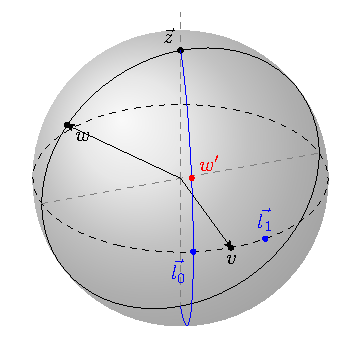
\includegraphics[width=\textwidth]{construction.pdf}
    \caption{Procedure on $S^2$.}
  \end{subfigure}
  \hfill
  \begin{subfigure}[b]{.4\textwidth}
    \centering
    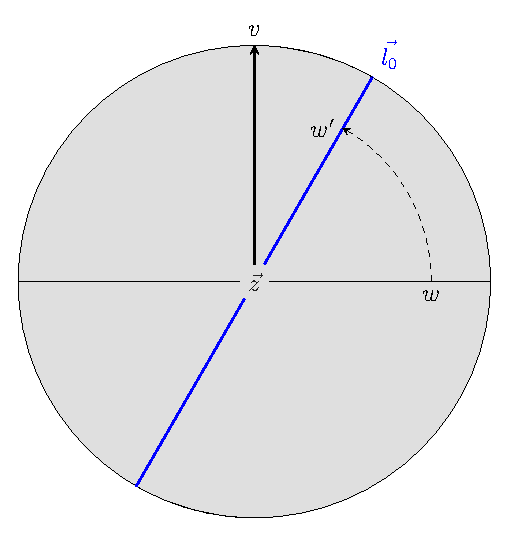
\includegraphics[width=\textwidth]{xy.pdf}
    \caption{Projection on the $xy$-plane.}
  \end{subfigure}
  \caption{Construction of $h_3$.}
  \label{fig:planes}
\end{figure}

The direction $w'$ defines an oriented linear plane $P = \left\{ p\in \bbR^3 \vert \scalar{w'}{v} =0\right\} $ that is orthogonal to $h_0$ by construction, thus the projection of $\mu$ on $p$ is bisected by $p\cap h_0$.
By Ham-Sandwich theorem there is a (unique) line $\gamma$ that splits the two halves simultaneously, define $h_2$ to be the affine span of $w'$ and $\gamma$.

In particular, we have constructed a continuous map $\phi:E\rightarrow \left(S^3\right)^3$:
\[
(v,w) \mapsto (h_0(v), h_1(v), h_2(v, w))
\]
with $E$ the $S^1$-bundle over $S^1$ defined as
\[
E = \left\{ (v, w) \in S^2\times S^2 \ \vert \  v_3 = 0 \mbox{ and } \scalar{v}{w} = 0\right\}.
\]

It is possible to define a $G$ action on $E$ as follows:
\begin{align*}
  \nu_1((\matrice{v_1\\v_2\\v_3}, \matrice{w_1\\w_2\\w_3})) = (\matrice{-v_1\\-v_2\\-v_3}, \matrice{-w_1\\-w_2\\w_3})\\
  \nu_{2}((\matrice{v_1\\v_2\\v_3}, \matrice{w_1\\w_2\\w_3})) = (\matrice{v_1\\v_2\\v_3}, \matrice{-w_1\\-w_2\\-w_3})
\end{align*}

It is straightforward to verify that, if we fix the action of $G$ on $\left(S^3\right)^3$ to be the one induced by the subgroup of $\left(\ztwo\right)^3 = \langle \eta_1, \eta_2,\eta_3\rangle$ generated by $\eta_1 + \eta_2$ and $\eta_3$, then the map $\phi$ is $G$-equivariant.
\vskip 1em
Any plane arrangement $\mathcal{H}$ is an equipartition if and only if all the signed sums $f_\alpha$ are $0$, however, all the signed sums beside $f_{(1,1,1)}$ and $f_{(0,1,1)}$ are $0$ for any arrangement obtained through the previously outlined construction.

Thus, $\mathcal{H}$ equipartitions $\mu$ if and only if the $G$-equivariant map in $\bbR^2$
\[
f(\mathcal{H}) = \left(f_{(1,1,1)}(\mathcal{H}), f_{(0,1,1)}(\mathcal{H})\right)
\]
has a $0$.


The last thing left to check is that the configuration space is indeed $G$-homeomorphic to the standard torus $T^2= S^1\times S^1$.

However, it is possible to define an explicit $G$-isomorphism $\psi:T^2\rightarrow E$:
\[
(\phi, \theta) \mapsto
(\begin{pmatrix}
\cos(\phi)\\
\sin(\phi)\\
0
\end{pmatrix}
\begin{pmatrix}
\sin(\theta)\sin(\phi)\\
-\sin(\theta)\cos(\phi)\\
\cos(\theta)
\end{pmatrix})
\]

The $G$-map is continuous, injective, surjective and closed $\Rightarrow$ it is a $G$-homeomorphism.

\section{Equivariant topology}

\begin{theorem}
  Let $f:T^2 \rightarrow_G \bbR^2$. Then $f$ has a zero.
\end{theorem}

\vskip 1em
\noindent
\textbf{First Proof: fundamental group obstruction}
\hrule
\vskip 1em

\begin{proof}
  By contradiction, suppose $\exists f: T^2 \rightarrow_G \bbR^2\setminus \{0\} \sim S^1$. Then $f$ induces a map on the level of fundamental groups:

  \[
    f_*: \pi_1(T^2) \simeq \bbZ^2 \rightarrow \pi_1(S^1)\simeq\bbZ
  \]

\vskip 1em
Denote by $\mu, \lambda$ the usual generators for $\pi_1(T^2)$ (see figure \ref{fig:generators}) and by $\gamma$ the class of the identity in $\pi_1(S^1)$.

\begin{figure}[hbt]
  \centering
  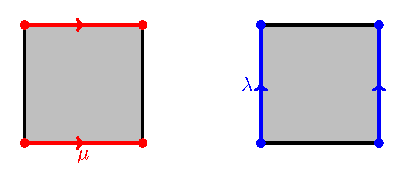
\includegraphics[width=\textwidth]{pic.pdf}
  \caption{Representatives for the generators.}
  \label{fig:generators}
\end{figure}

Using the generators, we can explicitly compute the action of $G$ on both the fundamental groups:

\vskip 1em

\begin{tabularx}{0.8\textwidth} {
    >{\centering\arraybackslash}X
  | >{\centering\arraybackslash}X }
Action on $\pi_1(T^2)$ & Action on $\pi_1(S^1)$\\
\hrule & \hrule\\

Trivial, i.e. & $\nu_1^S(\gamma) = -\gamma$ \\
$\nu_1^T=\nu_2^T=Id$ & $\nu_2^S(\gamma) = \gamma$ \\
\end{tabularx}
\vskip 1em

The group homomorphism $f_*:\bbZ^2 \rightarrow \bbZ$ is completely determined by the images $f_*(\lambda) = n \gamma$ and $f_*(\mu) = m \gamma$.

Since $f_*$ is $G$-equivariant we have:

\[
  n\gamma = f_*(\lambda) = f_*(\nu_1^T(\lambda)) = \nu_1^S(f_*(\lambda)) = -n\gamma \Rightarrow n = 0
\]

On the other hand, by checking what happens along the diagonal $\lambda + \mu$ we have:

\[
  m\gamma = f_*((\nu_1^T\nu_2^T)(\lambda + \mu)) = (\nu_1^S\nu_2^S)(f_*(\lambda + \mu)) = -m \gamma \Rightarrow m=0
\]

However, we can map $S^1$ on the torus $g:S^1 \rightarrow S^1\times S^1$, $g(\theta) = (0, \theta)$ such that $g$ is an antipodal map, i.e. $g(\pi+\theta) = \nu_1^T(g(\theta))$.
The composition $fg:S^1 \rightarrow S^1$ is an antipodal map on $S^1$ $\Rightarrow$ $deg(fg)$ is odd, but $deg(fg) = 0$ since $f_*$ is identically $0$.

\end{proof}

\vskip 1em
\noindent
\textbf{Second Proof: Fadell-Husseini index}
\vskip .2em
\hrule
\vskip 1em

\begin{proof}

  The target space $\bbR^2$ is $G$-isomorphic to the representation $V_{01}\oplus V_{11}$ and thus $S(\bbR^2) = S(V_{01})*S(V_{11})$.
  Fixing $\bbF_2$ as coefficients we have that:

\begin{align*}
  Ind_G(V_{(\alpha_0, \alpha_1)}) = (\alpha_0 t_0 + \alpha_1 t_1) \subseteq \bbF_2\left[ t_0, t_1\right] \\
  Ind_G(X)Ind_G(Y)\subseteq Ind_G(X*Y)
\end{align*}

As a consequence $(t_0t_1 + t_1^2)\subseteq Ind_G(S(\bbR^2))$; however:
\[
  t_0t_1 + t_1^2 \notin (t_0^2, t_1^2) = Ind_G(S^1\times S^1) \Rightarrow Ind_G(S(\bbR^2)) \nsubseteq Ind_G(S^1\times S^1)
\]

Thus, there is no $G$-equivariant map $S^1\times S^1 \rightarrow S(\bbR^2)$.
\end{proof}

\vskip .5em
\subsection{Explicit construction of the test map}

The purpose of this section is to explicitly define and check the symmetries of the map:

\[
  \Phi: E \rightarrow \left(S^3\right)^3
\]

In order to simplify a bit the notation, we will denote by $\overline{x} = \frac{x}{\lVert x\rVert}$ the normalization of a non-zero vector $x$.

\vskip 2em
\noindent
\textbf{Construction of the map}
\hrule
\vskip 1em

Given a point $(v, w)\in E$, the bisecting lines for the projected mass on the horizontal plane are going to be defined as $l_0 =\bbR \vec{l_0}(v) + b_0(v) $
(with $\vec{l_0}, b_0 \in \bbR^3$). The vector $\vec{l_0}$ is defined as the unique vector of length one spanning the linear part of $l_0$ such that
such that $z = \overline{(\vec{l_0}\wedge v)}$ (equivalently, $\vec{l_0}$ is the first one contraclockwise from $v$)\footnote{Both $v$ and $\vec{l_0}$ are always orthogonal to $z$
by construction so the only possible case where the definition doesn't make sense is where $\vec{l_0} = \pm v$; however, if this was the case, the
lines $l_0$ and $l_1$ would coincide and thus wouldn't be bisecting the projected problem.}.

In particular, the plane $H_0 = \langle \vec{l_0}, z\rangle + b_0$ has a natural orientation defined by the direction $z\wedge \vec{l_0}(v)$
and it induces a well defined point $h_0 \in S^3$:
\[
  h_0(v) = \overline{\matrice{ z \wedge \vec{l_0}(v) \\ \scalar{b_0(v)}{(z\wedge\vec{l_0}(v))}}} \in S^3
\]
The plane $H_1$ and the point $h_1$ are constructed in the same way using the line $l_1$.


Let now $P$ be the linear oriented plane defined by $w' = R_v(w)$ (i.e. the plane orthogonal to $w'$ with the induced orientation) and $\lambda$
be the affine line corresponding to the projection of $H_0$ on $P$; by construction $\lambda= H_0 \cap P$, thus it has a natural orientation.
Denote its direction by $\vec{\lambda}$.

By Ham-Sandwich theorem, there is a unique $\gamma = \bbR y(v, w) + c(v, w)\subseteq P$ line (with $y, c\in \bbR^3$) that,
together with $\lambda$, split the projected mass in $4$ equal pieces.
The vector $y$ is the unique vector of length $1$ such that $\overline{\vec{\lambda}} \wedge y = w'$ and $y$ spans the linear part of $\gamma$.

Finally, the plane $H_2$ spanned by $\gamma$ and $w'$ has a natural orientation, induced by the normal $y\wedge w'$ and thus it defines
a point $h_2$ in $S^3$:
\[
  h_2(v, w) = \overline{\matrice{y(v, w)\wedge w'\\\scalar{c(v,w)}{(y(v,w)\wedge w')}}}.
\]

The map is thus the following:
\[
  \left(v, w\right) \mapsto \left( h_0(v), h_1(v), h_2(v, w)\right)
\]

All the constructed lines depend continuously on $v, w$ and the mass $\mu$ and since the orientation can be chosen consistently,
the total map is well defined and continuous.

\vskip 2em
\noindent
\textbf{Symmetries}
\hrule
\vskip 1em

The space $E$ has the natural product $G$-action:
\begin{align*}
  \nu_1^E(v, w) = (-v, w) \\
  \nu_2^E(v,w) = (v, -w)
\end{align*}

\textbf{DANGER:} This action is NOT the same as the action described in the previous section! This causes problems.

\begin{lemma}
  Suppose $\Psi(v,w) = (h_0, h_1, h_2)$, then:
  \begin{align*}
    \Psi(\nu_1^E(v, w)) = (-h_0, -h_1, -h_2) \\
    \Psi(\nu_2^E(v, w)) = (h_0, h_1, -h_2)
  \end{align*}
\end{lemma}
\begin{proof}
  If we swap $v$ with $-v$ in the construction, the vector $\vec{l_0}$ keeps the same direction but changes sign, i.e. $\vec{l_0}(-v) = -\vec{l_0}$.
  Since $b_0$ is the translation vector, this is not changed and so $h_0(-v) = -h_0(v)$ (the same reasoning works for $h_1$ as well).

  Since both $v$ and $\vec{l_0}$ change sign, the rotation $R_v$ still maps the orthogonal meridian to the one containing $\vec{l_0}$,
  $w'$ does not change; as a result, the plane $P$ does not change orientation. However, $h_1$ has the opposite orientation and thus the
  line $\lambda$ swaps orientation as well.

  As a consequence, the vector $y$ for the new problem changes sign (the sign of $y$ is defined by the equation $\overline{\vec{\lambda}} \wedge y = w'$,
  where $\vec{\lambda}(-v) = -\vec{\lambda}(v)$ and $w'(-v) = w'(v)$).

  Overall, we have that $\Psi((-v, w)) = (-h_0, -h_1, -h_2)$.

  The other case is straightforward: $h_0$ and $h_1$ do not depend on $w$ so they are not changed; on the other hand,
  $w'(v, -w) = R_v(-w) = -w'(v,w)$ and thus the plane $P$ changes orientation. As a result, $\vec{lambda}$ changes sign and thus $y$ doesn't.

  Overall, since $w'$ changes sign and $y$ doesn't, we have that  $\Psi((v, -w)) = (h_0, h_1, -h_2)$.
\end{proof}

\section{Error in the proof}

The construction is wrong: the action on the torus $T$ that we need in order for it to be $G$-homeomorphic to $E$ is the following:
\begin{align*}
  \nu^T_1(\phi, \theta) = (\phi + \pi, 2\pi + \theta) \\
  \nu^T_2(\phi, \theta) = (\phi, \pi + \theta)
\end{align*}

The issue is that there is no homotopic obstruction to having a $G$-map from the torus to $\bbR^2$; in fact, there exist such map:
\[
  (\phi, \theta) \mapsto (\cos(\theta), \sin(\theta))
\]

It is still worth noting that every isolated step of the previous proof is correct; in particular the construction of the affine planes with prescribed intersection outlined in section \ref{sec:torus_conf_space}.


\section{Order 4 symmetries}
Denote by $H$ the group $\bbZ_4\times \ztwo$.

The goal of this section is to construct a different set up of configuration space - test map, where the
objects involved are going to be $H$-equivariant.

\subsection{Configuration space-Test map setup}

Without loss of generality, we can assume the direction of the desired intersection to be $\vec{z}$. Fix now
a vector $v\in S^1$, by the same reasoning of section \ref{sec:torus_conf_space}, it is possible to construct
two  affine oriented planes $H_0$ and $H_1$ that split the measure equally, have the desired intersection and
depend continuously on $v$ (denote by $h_i$ the corresponding points on $S^3$).

It is also worth noting that, if $g_1^{S^1}$ is a rotation by $\frac{\pi}{2}$ clockwise of $S^1$, then by uniqueness of the cuts on the plane we have:

\begin{align*}
  h_0(g_1^{S^1}(v)) = -h_1(v)\\
  h_1(g_1^{S^1}(v)) = h_0(v)
\end{align*}

Now, fix $w\in S^2$; there exists a unique affine plane $H_2$ orthogonal to $w$ (oriented consistently with $w$)
that bisect the mass. Thus the point $h_2(w)\in S^3$ is well defined, depends continuously on $w$ and is such that
$h_2(-w) = - h_2(w)$.

\vskip 1em
By construction, all the planes split the mass in half and $H_0, H_1$ split the measure in equal parts.
Thus, the plane arrangement defined by $\mathcal{H}(v, w) = (h_0(v), h_1(v), h_2(w))$ is an equipartition if and only if:

\[
  \left\{
    \begin{aligned}
      f_{(1,1,1)}(\mathcal{H}) = 0 \\
      f_{(0,1,1)}(\mathcal{H}) = 0 \\
      f_{(1,0,1)}(\mathcal{H}) = 0 \\
    \end{aligned}
  \right.
\]

Denote by $g_2^{S^2}$ the antipodal action on $S^2$; then the following relations hold:

\begin{align*}
  f_{(1,1,1)}(\mathcal{H}(g_1^{S^1}v, w)) &= - f_{(1,1,1)}(\mathcal{H}(v, w))  \\
  f_{(0,1,1)}(\mathcal{H}(g_1^{S^1}v, w)) &= f_{(1,0,1)}(\mathcal{H}(v, w)) \\
  f_{(1,0,1)}(\mathcal{H}(g_1^{S^1}v, w)) &=  - f_{(0,1,1)}(\mathcal{H}(v, w))\\
\end{align*}

\begin{align*}
  f_{(1,1,1)}(\mathcal{H}(v, g_2^{S^2}w)) &= - f_{(1,1,1)}(\mathcal{H}(v, w))  \\
  f_{(0,1,1)}(\mathcal{H}(v, g_2^{S^2}w)) &= - f_{(0,1,1)}(\mathcal{H}(v, w))  \\
  f_{(1,0,1)}(\mathcal{H}(v, g_2^{S^2}w)) &= - f_{(1,0,1)}(\mathcal{H}(v, w))  \\
\end{align*}

In particular, if we fix the following action of $H = \langle g_1, g_2\rangle$ on $\bbR^3$:
\begin{align*}
  g_1^{\bbR}(x, y, z) &= (-x, z, -y)\\
  g_2^{\bbR}(x, y, z) &= (-x, -y, -z)
\end{align*}

and we define

\[
  F(v, w) = \matrice{f_{(1,1,1)}(\mathcal{H}(v,w))\\ f_{(0,1,1)}(\mathcal{H}(v,w))\\ f_{(1,0,1)}(\mathcal{H}(v,w))}
\]
then, we have that we have constructed an $H$-map $F:S^1\times S^2 \rightarrow \bbR^3$ whose zeros
correspond to equipartition with the desired intersection.

\subsection{Equivariant topology}

The goal of this section is to show the following result:

\begin{theorem}
  Let $F:S^1\times S^2 \rightarrow_H \bbR^3$. Then $F$ has a zero.
\end{theorem}

\begin{proof}
  By contradiction, suppose there exists a map $F$ that does not hit $0$; up to normalizing, we have a map
  $F: S^1\times S^2 \rightarrow_H S^2$.

  Given a point $a\in S^1$, fixing the first coordinate $F_a \equiv F(a, \bullet)$ defines an element in $\pi_2(S^2)$
  and any two such maps are homotopic\footnote{Given $a= e^{i\theta}$ and $b=e^{i\phi}$, the homotopy is given by
    $H(t, x) = F(e^{i(t\phi + (1-t)\theta)}, x)$.}; as a result, let $d$ be the degree of any such map.

  Fix now a point $a\in S^1$ and let $b=g_1^{S^1}(a)$. Then, $F_b(x)=g_1^{\bbR}(F_a(x))$ by $H$-equivariance, but
  this implies that:

  \[
    d[Id] = [F_b] = [g_1^{\bbR}\circ F_a] = \det(g_1^{\bbR})[F_a] = - [F_a] = -d[Id]
  \]

  Thus $d = 0$ and $F_a$ is nullhomotopic. However, by $H$-equivariance, $F_a$ is an antipodal map from $S^2\rightarrow S^2$ and thus it can
  not be nullhomotopic by Borsuk-Ulam.
\end{proof}
\end{document}
